\chapter{THỰC NGHIỆM VÀ ĐÁNH GIÁ}
\ifpdf
    \graphicspath{{Chapter4/Chapter3Figs/PNG/}{Chapter4/Chapter4Figs/PDF/}{Chapter4/Chapter4Figs/}}
\else
    \graphicspath{{Chapter4/Chapter4Figs/EPS/}{Chapter4/Chapter4Figs/}}
\fi

\markboth{\MakeUppercase{\thechapter. My Fourth Chapter }}{\thechapter. THỰC NGHIỆM VÀ ĐÁNH GIÁ}
 
 	Để hiểu rõ hơn về phương pháp và đánh giá độ chính xác của mô hình đã trình bày ở trên. Trong chương này sinh viên sẽ tiến hành chạy thực nghiệm các mô hình trình CNN, Hydra CNN cho ba bộ dữ liệu TRANCOS, UCSD và UCF. Từ kết quả thu được sinh viên sẽ tiến hành so sánh với các phương pháp khác đã được đề xuất và bên cạnh đó sẽ xây dựng một công cụ mô hình hóa trực quan dữ liệu nhằm tìm ra những ưu điểm và hạn chế của phương pháp. Để từ đó đặt ra những giả thiết cho các vấn đề còn tồn tại của phương pháp. 
\section{Bộ dữ liệu thực nghiệm.}

	Trong phạm vi khóa luận này, sinh viên tiến hành đánh giá trên ba bộ dữ liệu tương ứng với ba tiêu chuẩn đánh giá. trong đó, hai bộ được sử dụng để đánh giá cho bối cảnh đám đông: bộ UCSD (dữ liệu người đi bộ), và $UCF\_CC\_50$ (dữ liệu đám đông mật độ lớn). Và bộ còn lại là bộ dữ liệu TRANCOS để đánh giá cho bối cảnh đếm các phương tiện giao thông trong các bối cảnh giao thông tắc nghẽn.

\subsection{Bộ Dữ liệu UCSD}
	UCSD \cite{chan2008privacy} là mộ bộ dataset phổ biến thường được sử dụng để đánh giá cho các phương pháp liên quan đến phân tích người đi đi bộ. Bộ dữ liêu này được thu thập từ một camera giám sát cố định đặt ở lối đi dành cho người đi bộ ở đại học California, San Diego với một giờ dữ liệu video. Video gốc được ghi với tốc độ 30 fps và kích thước mỗi frame là $740 \times 480$, sau đó dữ liệu được hạ xuống 10 fps và kích thước còn $238 \times 158$ mội frame. Với 2000 frame đầu tiên (200 giây dữ liệu video) được gán nhãn ground true với tổng số 49,855 nhãn được dán.  Các hình này được gán nhãn bằng cách gán một dấu chấm đại diện cho mỗi người đi bộ, và một khu vực tính toán (ROI - Region of Interest) được đánh dấu trên mỗi ảnh. 
	
\subsection{Bộ dữ liệu $UCF\_CC\_50$}
	Đây là một bộ dữ liệu chứa hình ảnh đám đông với mật độ lớn. Được thu thập chủ yếu từ FLICKR với mục đích cung cấp dữ liệu cho nghiên cứu đám đông (minh hoa trong hình \ref{ucf} \footnote{http://crcv.ucf.edu/data/crowd\_counting.php}). Bộ dataset này bao gồm 50 bức ảnh đám đông chứa số người trong hình từ 94 đến 4543 người, và trung bình là 1280 người mỗi hình. Mỗi người được gán nhãn bằng một dấu chấm. Những hình ảnh này chứa cảnh cực kỳ đông đúc trong các bối cảnh như: các cuộc biểu tình, các sự kiện âm nhạc, Các sân vận động bống đá hay các sự kiện ngoài trời. Bộ dataset này dùng để đánh giá và kiểm chứng một thách thực quan trọng trong chủ đề đếm đối tượng khi mà số lượng đối tượng rất lớn cùng các khó khăn như sự che khuất, sự biến dạng do góc nhìn hay quá ít pixel biểu diễn cho một đối tượng. bên cạnh đó, số lượng hình ảnh để huấn luyện giảm đáng kể xuống còn rất ít (50 hình) và trong nhiều bối cảnh khác nhau xen lẫn trong bộ dữ liêu. Đó là những thách thức mà bộ dataset này đặt ra. \par 
	
\begin{figure}[ht]
  			\begin{center}
    				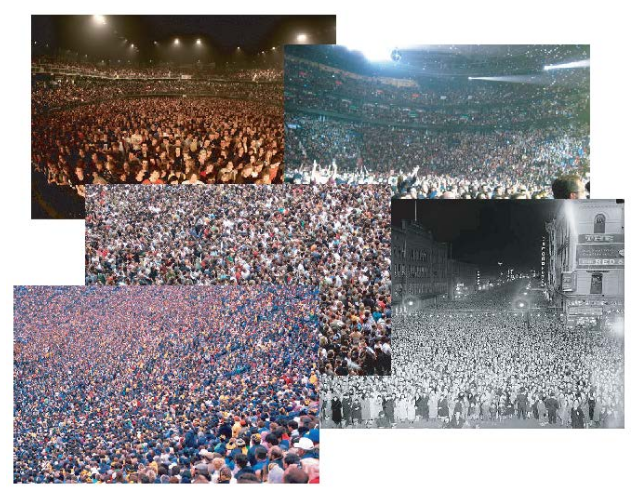
\includegraphics[scale=0.5]{ucf} 
    				\caption{một vài hình ảnh trong bộ dữ liệu UCF}
    				\label{ucf}
  			\end{center}
\end{figure}	

\subsection{Bộ dữ liệu TRANCOS}
	Bộ dữ liệu TRANCOS (TRaffic ANd COngestionS) \cite{guerrero2015extremely} là một dataset dùng để đánh giá tiêu chí các đối tượng bị che khuất lớn của các phương tiện giao thông trong bối cảnh giao thông tắc nghẽn. Bộ dataset bao gồm 1244 hình ảnh được thu thập từ các camera giám sát giao thông thực tế ở thành phố Dirección General de Tráfico Tây Ba Nha. Với tổng số 46796 nhãn phương tiện giao thông. Các phương tiện giao thông được gán nhãn trực tiếp bằng tay bằng các dấu chấm đại diện cho mỗi phương tiện. Và kèm theo đó cung cấp thêm vùng tính toán quan tâm (ROI) tương tự như bộ UCSD cho mỗi hình ảnh. Bộ dữ liệu này cung cấp các hình ảnh chứa các bối cảnh rất đa dạng và hơn thế nữa là các camera còn có nhiều góc nhìn khác nhau trong cùng một cảnh. \par 
  
\section{Phương pháp đánh giá thực nghiệm.}
	Trong phần này, sinh viên sẽ tiến hành chạy thực nghiệm đánh giá hai mô hình CCNN và Hydra CNN trên ba bộ dữ liệu kể trên (UCSD, UCF, TRANCOS). Mỗi bộ dữ liệu sẽ có hình thức đánh giá riêng theo yêu cầu của mỗi dataset cùng các độ đo áp dụng cho mỗi bộ. Sau đây sinh viên sẽ trình bày chi tiết quy trình đánh giá thực nghiệm.
\subsection{Đánh giá thực nghiệm trên bộ UCSD} 
	Với bộ dataset UCSD, sinh viên thực hiện quá trình thực nghiệm với cách phân chia dữ liệu sử dụng trong \cite{onoro2016towards,zhang2015cross,lempitsky2010learning,fiaschi2012learning,
	ryan2009crowd}. Bộ dữ liệu được chia thành bốn tập khác nhau để huấn luyện, và tất cả các frame còn lại trong mỗi tập được dùng để test.
	\begin{itemize}
		\item Maximal: được huấn luyện với các frame 600:5:1400
		\item downscale: huấn luyện với các frame 1205:5:1600
		\item upscale: huấn luyện với các frame 805:5:1100
		\item minimal: huấn luyện với các frame 640:80:1360
	\end{itemize}	
	
	Trong quá trình huấn luyện cho mô hình CCNN, với mỗi frame hình ảnh, ta tiến hành rút trích ra 800 patch ngẫu nhiên trên toàn bộ hình ảnh với kích thước $72 \times 27$ pixel. sau đó ta lại lật mỗi patch $180^o$ với mục đích tăng số lượng dữ liệu huấn luyện. Cuối cùng, ta thu được tổng cộng 1600 mẫu dữ hiệu huấn luyện với mỗi hình. Những patch với kích thức $72 \times 72 $ sẽ là đầu vào cho mô hình mạng. Kèm với đó, ta sẽ tạo bản đồ mật độ ground truth bằng phương pháp được sử dụng trong \cite{lempitsky2010learning}. Ở đây, ta tính toán Gaussian Kernel (với ma trận hiệp phương sai (covariance matrix) $\sum = 8.1_{2x2}$) tại điểm chính giữa của mỗi nhãn đối tượng.\par
\begin{figure}[ht]
  			\begin{center}
    				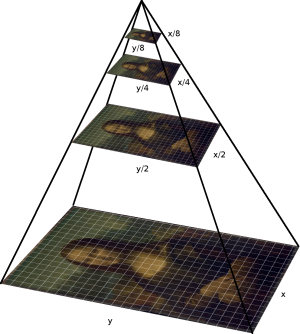
\includegraphics[scale=0.7]{pyramid} 
    				\caption{Mô hình Pyramid với nhiều tỉ lệ trên một patch.}
    				\label{pyramid}
  			\end{center}
\end{figure}	
	Để huấn luyện cho mô hình Hydra CNN, ta vẫn sẽ tiến hành theo phương pháp trích xuất các patch được sử dụng trong mô hình CCNN. Điểm khác ở đây chính là với một patch thu được, ta sẽ giải quyết vấn đề tỉ lệ bằng cách áp dụng nhiều tỉ lệ khác cho một patch huấn luyện. Ta xây dựng một mô hình Kim tự tháp (pyramid) với s tỉ lệ khác nhau. Cụ thể hơn, tầng đầu tiên của mô hình Pyramid chưa patch với kích thước ban đầu. Nhưng đến tâng tiếp theo, ta sẽ lấy ra patch từ chính giữa tâm của patch ban đầu với tỉ lệ bằng $\dfrac{1}{s}$ kích thước của patch ban đầu. Ví dụ, trong trường hợp với mô hình Hydra CNN với hai đầu, tần đầu tiên chứa patch hình góc ban đầu. và tầng thứ hai chứa patch với kích thước bằng $50\%$ kích thước patch ban đầu. Vì vậy, với 800 patch được trích xuất ngẫu nhiên trong bức hình có kích thước $72 \times 72$ pixel. Sau đó tiến hành lấy ra pyramid của mỗi patch như mô tả ở trên. Cuối cùng, khi thu được mô hình cùng bộ tham số cuối cùng, ta sẽ kiếm tra mô hình trên dữ liệu test. Với mỗi hình test, ta sử dụng cửa sổ kích thước $10\times10 $ pixel trượt qua toàn bộ hình ảnh để tính toán cho toàn bộ ảnh. Dưới đây là một số hình ảnh chạy thực nghiệm kiểm tra với độ sai số ít nhất trên bộ dữ liệu (). 

\begin{figure}[ht]
  			\begin{center}
    				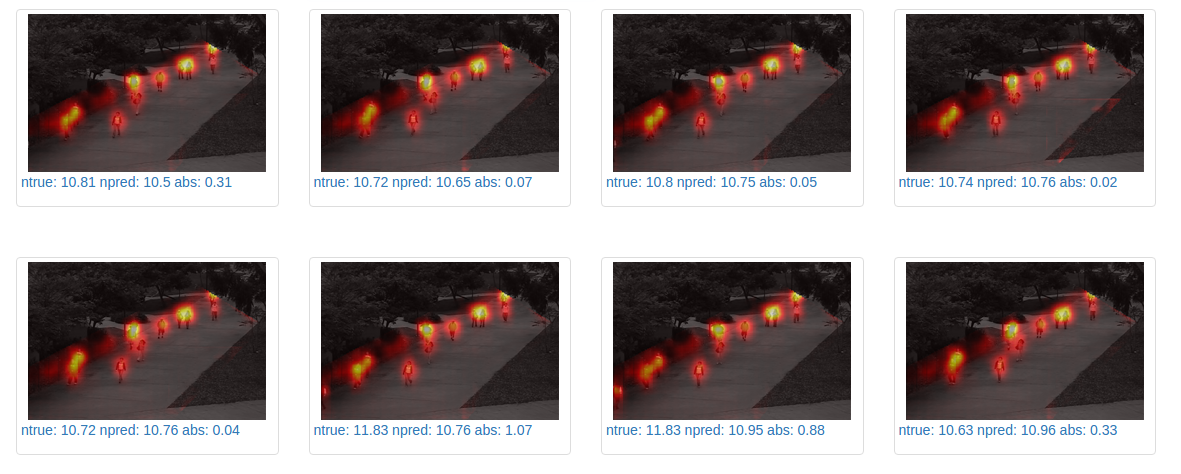
\includegraphics[scale=0.35]{ucsd} 
    				\caption{Mộ số ví dụ trong bộ dữ liệu test sau khi chạy thực nghiệm với kết quả thể hiện gồm ground truth, kết quả dự đoán và giá trị sai lệch.}
    				\label{ucsd}
  			\end{center}
\end{figure}	  
	

\subsection{Đánh giá trên bộ dữ liệu UCF} 
	
\subsection{Đánh giá trên bộ dữ liệu TRANCOS}
	Đối với bộ Dữ liệu TRANCOS, sinh viên tiến hành thực hiện đúng theo các chỉ định cài đặt thực nghiệm được sử dụng trong 
\section{Kết quả đánh giá}

\subsection{Kết quả đánh giá trên bộ dữ liệu UCSD}

\subsection{Kết quả đánh giá trên bộ dữ liệu UCF} 

\subsection{Kết quả đánh giá trên bộ dữ liệu TRANCOS}